\title{Git Assignment}
\author{Christopher Colvin}
\date{September 25, 2023}

\maketitle

\section{Introduction}
\subsection{Goals For CS6000}
\paragraph{\quad I intend to learn how to write research papers. In the research papers being written, I would implement my own previous research projects valid and verifiable through understanding what research is. I would like to network with others to critique and improve my current research interests, and use professional tools to identify possible allies for developing research together. Many projects I have worked on and share for academic purposes are considered research to my recent colleagues with their doctoral degrees. This provides me hope to learn in this course alongside having an advantage to develop previous works into research papers to start my career off strong. I really appreciated our class on 8/22/2023, the highlight was identifying the strong potential to earn a strong reputation from UCCS, as opposed to Harvard, with the determinant for employability being our abilities to publish or perish. I believe in learning from anyone, anywhere. Learned hard and soft skills at UCCS will yield positive progress if recipients are willing to put in the effort. The hard skills will be to recognize ideas relevant for research, begin researching the topic, effectively and efficiently document the research, and publish the findings with the ability to be reproducible.}
\subsection{What I Hope To Learn}
\paragraph{\quad I hope to learn the upper and lower bounds of criteria for identifying relevant ideas/concepts to research. In our class on 08/22/2023, I understand using Google Scholar to primarily identify if the concept is novel or previous research has not occurred is optimal. The secondary priority appears to be measuring the societal impact of the idea/concept. The depth/width of the concept are currently two components to assess the societal impact. I now understand one significance of this measurement identifies private algorithms/processes and private data as being effectively an 
“island” of knowledge that will not be authorized for sharing. The possibility of algorithms to be protected in a patent relevant to National Security is permitted by the Invention Secrecy Act of 1951. In class, the combination of a public algorithm/process, but use with private data is still considered a slippery slope for research. I understand the security implications with sharing an algorithm used for private data, as the input data can be inferred by the algorithms used to analyze it. I also understand the limited societal impact by relying on private data, or such a specific dataset. The factors I really look forward to measuring combinations of scales for certain bounds (not limited to), broad versus narrow societal application, profound versus mild depth, novel versus known, and problem versus solution. I also hope to learn the ability to identify the audience level and language to use in specific research papers. The current learned strategy from 08/22/2023 is to utilize Google Scholar to identify relevant and related publications, which helps bridge the language gap I seek. The audience level continues to elude me at this time 08/26/2023.}
\subsection{Degree I Am Studying}
\paragraph{\quad I am pursuing the Computer Science PhD in Security}
\subsection{Something Personal}
\paragraph{\quad I enjoy working with systems in general, such as restoring classic cars. I also specialize in identifying novel processes or process optimization methods, such as developing automotive tire and exhaust efficiency calculations and optimizations.}
\subsection{My Photo As A  Figure}
\paragraph{\quad Please see the next page for my picture.}
\begin{figure}[ht!]
\centering
\caption{\label{fig:CColvin_Headshot} My photo, it has also been posted to Canvas during this exercise on 08/26/2023.}
\includegraphics[width=0.8\textwidth, height=1\textwidth]{CColvin_Headshot.jpg}
\end{figure}
\clearpage
\subsection{Testing Related Git Code}
\paragraph{\quad The credit for the original code is from DanNegrea on GitHub, link to the repo below (DanNegrea \textit{DanNegrea/Scapy-Interceptor: Intercept and edit packets on the fly.)}:}
\hfill \break
\href{https://github.com/DanNegrea/Scapy-Interceptor.git}
{Scapy-Interceptor}
\\
\url{https://github.com/DanNegrea/Scapy-Interceptor.git}

\paragraph{\quad For my network security research, this code allows for packet interception and on the fly modification to packet headers and data from any and all packets in a Linux system. I developed my own Man In The Middle attack code during penetration testing and will utilize this to extend this functionality and build a hybrid proxy server of sorts for my research. This code can use system packets as templates, replicate them, and test firewalls for different IP address and port combinations over time. This includes whether they are closed or not in the view of Nmap/Zenmap and other port scanning software. Please see the next page for a demo of intercepting a ping to Google, being changed to ping a different IP address (75 instead of 78). A different address error is present because of this, however this code remains a remarkable success. Other code used in the past only allowed crafted/controlled individual packets to be manipulated as opposed to any packet moving through the interface, with the ability to program filters.}
\clearpage
\begin{figure}[ht!]
\centering
\caption{\label{fig:CColvin2023-09-26 08 13 39} A demo of testing the relevant Git code, and successful results during this exercise on 09/26/2023.}
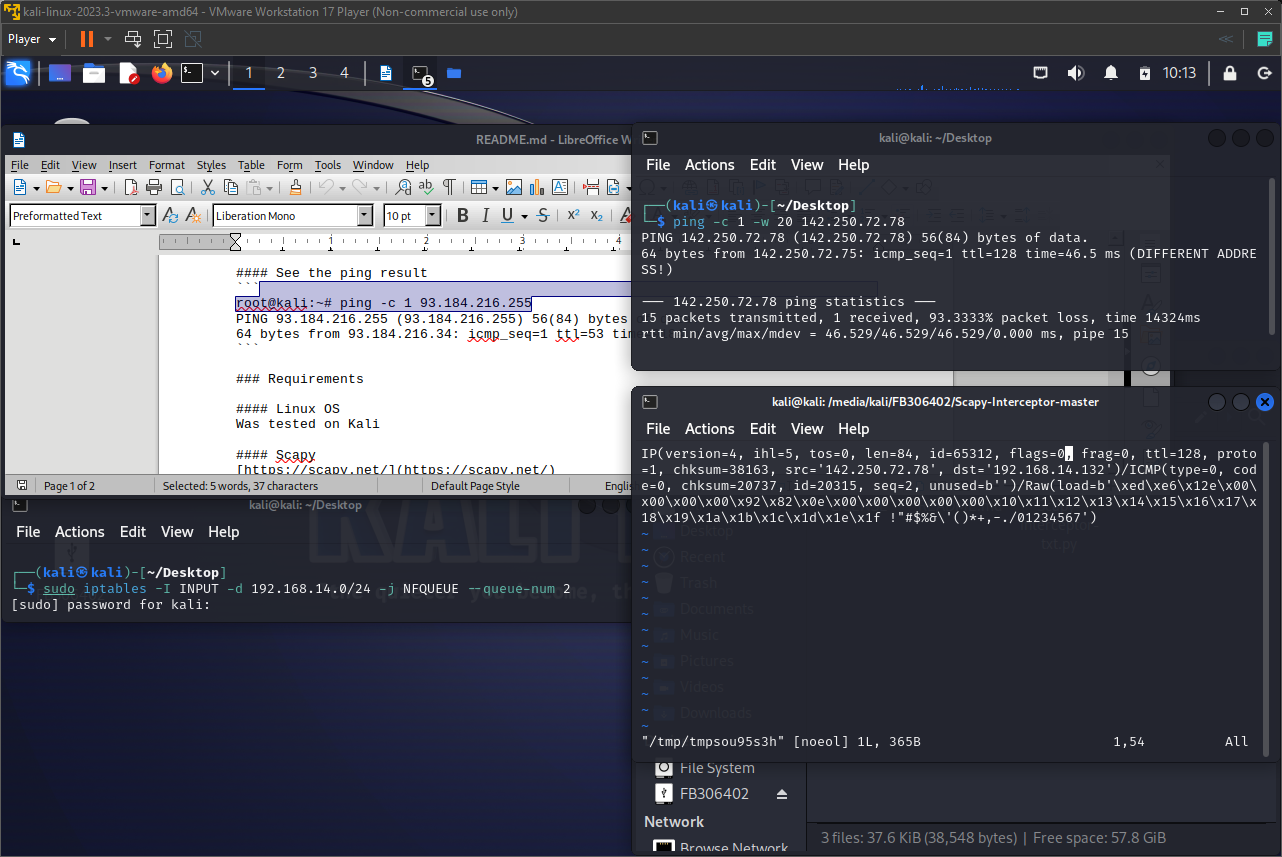
\includegraphics[width=1.35\textwidth, height=1\textwidth]{CColvin2023-09-26 08 13 39.png}
\end{figure}
\section{References}
\begin{enumerate}
    \item[] DanNegrea, Alias. “Dannegrea/Scapy-Interceptor: Intercept and Edit Packets on the Fly.” \textit{GitHub}, 25 Apr. 2019, github.com/DanNegrea/Scapy-Interceptor.git. Scapy and netfilterqueue on the fly packet interception and manipulation original code.
\end{enumerate}
